\chapter{Behavior of electromagnetic waves in space (lasers and slits)}

\section{Introduction}

In 1801, Thomas Young's ``double-slit'' experiment demonstrated the wave nature of light by showing that two coherent light sources produce interference patterns. You will perform a modern version of Young's experiment using a
laser as light source. The laser illuminates two thin slits, each of width $a$ separated by a distance $d$, which act as two
coherent sources of light. This is analogous to what you have observed with water waves in the previous lab section, in
which you saw a plane wave combined with an aperture (a slit) acting as a circular source of waves. An interference
pattern appears on a viewing screen, placed at a distance $L$ from the double slit, in the form of bright and dark regions
corresponding to maxima and minima of interference. You will use the interference pattern to measure the wavelength
$\lambda$ of the laser, and show that the same framework of equations that is derived in the introduction to the previous lab
holds for light too.

\section{Topic selection for individual paper and presentation}

By the end of lab today, ensure that you have chosen a topic for your individual project, and that it has been approved by your TA.

\section{Team roles}

\begin{steps}
	\item \textbf{Decide on roles} for each group member.
\end{steps}

The available roles are:

\begin{itemize}
	\item Facilitator: ensures time and group focus are efficiently used
	\item Scribe: ensures work is recorded
	\item Technician: oversees apparatus assembly, usage
	\item Skeptic: ensures group is questioning itself
\end{itemize}

These roles can rotate each lab, and you will report at the end of the lab report on how it went for each role. If you have fewer than 4 people in your group, then some members will be holding more than one role. For example, you could have the skeptic double with another role. Consider taking on a role you are less comfortable with, to gain experience and more comfort in that role.

Additionally, if you are finding the lab roles more restrictive than helpful, you can decide to co-hold some or all roles, or think of them more like functions that every team needs to carry out, and then reflecting on how the team executed each function.

\section{Add members to Canvas lab report assignment group}

\begin{steps}
	\item On Canvas, navigate to the People section, then to the ``Lab 2 Groups'' tab. Find a group that is not yet used, and have each person in your group add themselves to that same lab group.
\end{steps}

This enables group grading of your lab report. Only one person will submit the group report, and all members of the group will receive the grade and have access to view the graded assignment.

\section{Experiment 1: Observing patterns made by 1 and by 2 slits}\label{li:sec:exp1}

\subsection{Goal}

Describe the patterns made by a laser that is incident on 1 slit and on 2 slits, and the differences and similarities between them.

\subsection{Available equipment}

\begin{itemize}
	\item In this remote environment, imagine you have a laser, slit card, and screen as shown in Figure\ \ref{lir:fig:setup}.
\end{itemize}

\begin{figure}
	\centering
	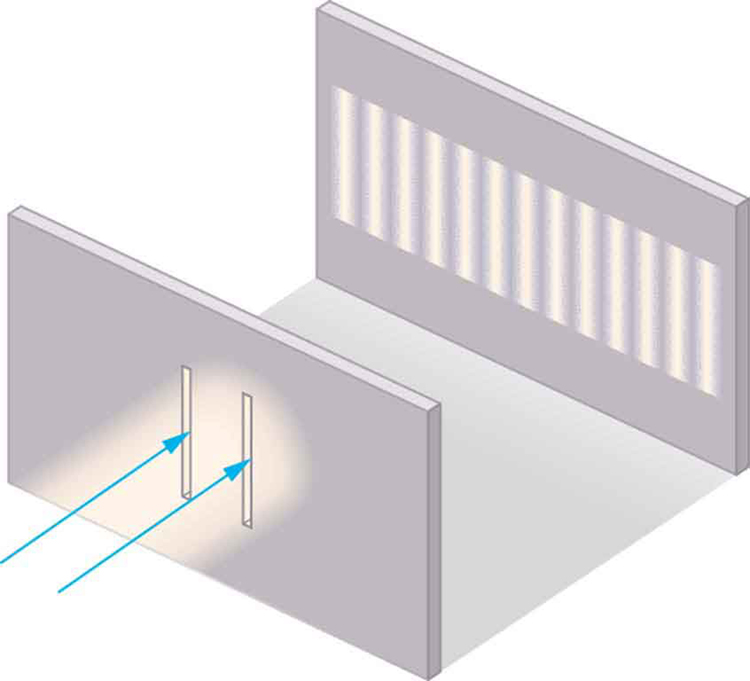
\includegraphics[width=0.5\textwidth]{laser-interference-remote/double-slit-setup.jpeg}
	\caption{Setup for the double-slit experiment. Laser light of a single frequency is sent through
		two slits and a pattern forms on the screen. Figure from OpenStax. Access for free at \url{https://openstax.org/books/college-physics/pages/27-3-youngs-double-slit-experiment}}\label{lir:fig:setup}
\end{figure}

\begin{figure}
	\centering
	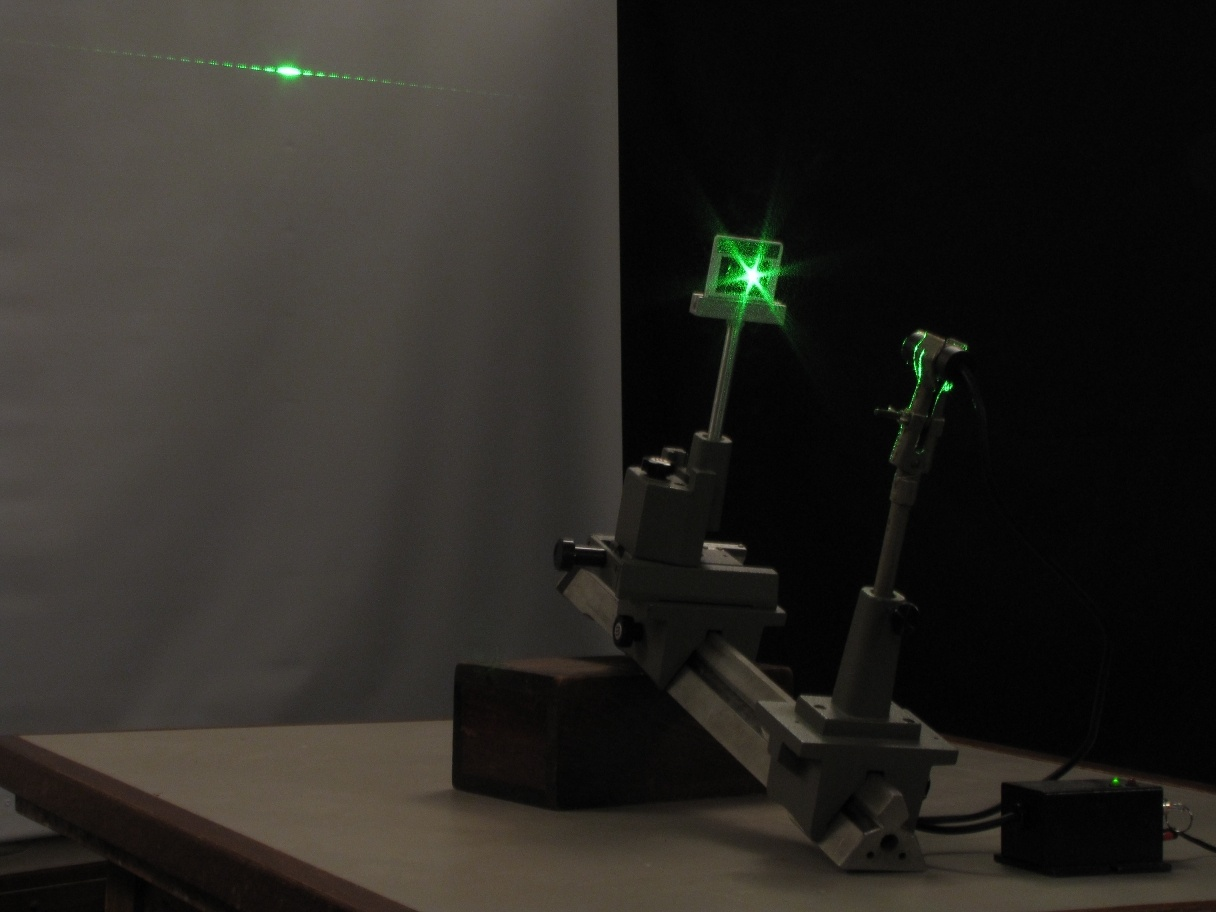
\includegraphics[width=0.5\textwidth]{laser-interference-remote/laser_double_slit_intererfence.JPG}
	\caption{Setup for the double-slit experiment. Laser light of a single frequency originates from the laser on the right. The laser light strikes the card in the middle, some of it passing through two thin vertical slits. A pattern forms on the screen. Image from \url{https://wiki.uchicago.edu/display/KER/Laser+Double+Slit+Interference} }\label{lir:fig:setup-photo}
\end{figure}

%optical bench, viewing screen, blank white paper, PASCO ``Multiple Slits'' assembly, red laser with mounting clamp, support stand, optionally computer with ImageJ installed

%\begin{framed}
%	\textbf{Warning: Laser Hazard!} The power of our lasers is low enough that the normal human blink reflex is sufficient to protect against incidental eye exposure.
%	
%	That being said, the following rules reduce the risk of eye exposure to laser light:
%	\begin{enumerate}
%		\item Do not direct the laser beam into anyone's eye.
%		\item Be aware of the laser reflecting off of mirror-like surfaces and where that beam goes.
%		\item Turn off the laser when not in use.
%		\item Keep the laser pointing horizontally and near the plane of the table, while keep your eyes above that plane.
%		\item To determine whether the laser is on, put your hand or a light-colored object in front of the beam, rather than looking into the laser aperture.
%	\end{enumerate}
%\end{framed}

\subsection{Rubrics to be assessed for this section}

F1, F2. See Appendix~\ref{cha:rubrics} for details.



%\subsection{Setup}
%Ensure the red laser is turned on and pointed at the slit assembly. Rotate the head of the slit assembly so that the active slit is the ''Comparison'' slit location with both a single
%and double slit furthest counter-clockwise. Adjust the laser so that the active slit
%is well illuminated by the laser spot. Note the laser should be pointed slightly upward if the laser head is ~10cm off the
%table, and pointed so it hits the screen ~5cm from the top edge, and so moving the slit assembly closer to the laser will
%move the spot on the slit assembly lower, and moving it further will move the spot higher. With the slits aligned with the
%laser, you will see light on the screen, but no longer a simple spot. Instead, you will see a vertical feature, the details of
%which depend on whether the laser is illuminating the single slit, or the double slit. Nudge the rail end back and forth to
%see the difference.

\subsection{Steps}

In our lab of the mind, we have a red laser sending a thin beam of light of a single wavelength through slits and onto a screen. A sketch of the situation is shown in Figure\ \ref{lir:fig:setup}, and a photo of the setup is shown in Figure\ \ref{lir:fig:setup-photo}. We first use just a single slit, and then use both of them. With the room lights off, we take a picture of each case. The results are shown in Figure\ \ref{lir:fig:patterns}.

\begin{figure}
	\centering
	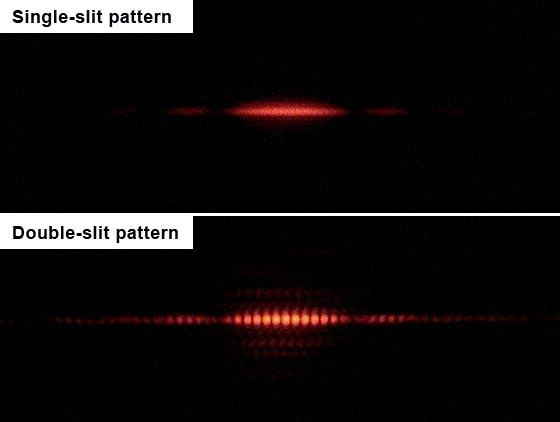
\includegraphics[width=0.6\textwidth]{laser-interference-remote/Single_slit_and_double_slit2.jpg}
	\caption{In a dark room, a laser is aimed at a card with a single or double slit in it. The light passes through the slit(s) and lights up a screen with the patterns shown. Image from \url{https://en.wikipedia.org/wiki/Double-slit_experiment\#/media/File:Single_slit_and_double_slit2.jpg}}\label{lir:fig:patterns}
\end{figure}

\begin{steps}
	\item Discuss the patterns observed in Figure\ \ref{lir:fig:patterns}. Describe each in detail. How are they alike and different? \textbf{Record your description and comparison.}
\end{steps}

\section{Experiment 2: Testing the wave hypothesis}\label{lir:sec:exp2}

\subsection{Goal}

Determine whether light from a laser can be described as a plane wave.

\subsection{Available equipment}

%Same as in Section~\ref{li:sec:exp1}, plus a green laser with mounting clamp

\begin{itemize}
	\item Simulation of laser light passing through slits, found at \url{https://physics.bu.edu/~duffy/HTML5/double_slit.html}
\end{itemize}

\subsection{Rubrics to be assessed for this section}

C4, C7, C8, G2, G4, F1, F2. See Appendix~\ref{cha:rubrics} for details.

\subsection{Behavior of a plane wave incident on single and double slits}

The following equation describes the location, $y_m$ (measured relative to the center of the pattern), of the $m$th interference \textit{minimum} (dark spot) seen on a screen when a plane wave is incident on a single slit.
\begin{equation}
y_m = \frac{m \lambda L}{a} \,,
\end{equation}
where $L$ is the distance from the slit to the screen, and $a$ is the width of the slit.

For a double slit, the following equation describes the location $y_n$ of the $n$th interference \textit{maximum} (bright spot) seen on a screen when a plane wave is incident on a double slit.
\begin{equation}
y_n = \frac{n \lambda L}{d} \,,
\end{equation}
where $d$ is the distance between the two slits. These equations use the same principle of path length difference as used in the previous lab, but are derived for the case where the distance from slit to screen is much larger than the slit and spacing dimensions.

\subsection{Suggestions for your experiment}

\begin{itemize}
	
%	\item \textbf{REQUIRED:} Use both the green laser and the red laser for this experiment, and ensure that you keep the data (image and setup parameters) for use in the individual homework.
	
%	\item For measuring the interference minima and maxima, you can do so by putting a paper on the screen and marking the locations directly, then measuring the marks with a ruler or with ImageJ. You could also take a picture of the pattern directly. Ensure that you take a reference photo with a known length on the screen, and take the image as face-on as possible, from the same location every time if you are taking multiple images.

	\item To get an uncertainty for your length measurements for the interference maxima and minima, you can have different teammates measure the same lengths and find the average and standard deviation.

%	\item The green laser has a wavelength of $532\:$nm. You can assume that this value is exact, with zero uncertainty.

	\item You can assume the values selected by the sliders are exact, with zero uncertainty.
	
%	\item The stated uncertainty in the slit size and separation according to the manufacturer (PASCO) is $\pm$ 0.005 mm for the slit width ($a$), and $\pm$ 0.01 mm for the slit spacing ($d$).
	
	\item If you use a value with an uncertainty in a calculation, if you want to use that value for comparison, you must propagate the uncertainty through to the final value. See Appendix~\ref{unc:sec:prop}.
	
	\item To compare your outcomes to your predictions, get a value with uncertainty for each, then compare them using the $t'$ test, described in Section~\ref{unc:sec:comparing}.
\end{itemize}

\subsection{Items to include in your report}

Relevant rubric rows from Appendix~\ref{cha:rubrics} are listed in parentheses.

\begin{enumerate}
	\item Statement of the hypothesis (C1).

	\item Description of the experimental setup and procedure (C2, F1).
	
	\item The quantitative prediction that the hypothesis makes about what will happen during the experimental procedure (C4). Ensure that uncertainty is handled correctly (G2).
	
	\item A report of the experimental outcome (results), neatly organized (G4).
	
	\item Determination of whether / how much the prediction agrees with the outcome, comparing using uncertainties (C7, G2).
	
	\item Judgment about the hypothesis --- based on this experiment, does it lead you to support the hypothesis more or less, about how much (qualitative)? (C8)
	
	\item A discussion of the findings of the experiment and why it's helpful (for you and/or for science) (F2).
\end{enumerate}

\section{Group functioning}

\begin{steps}
	\item Write a 100--200 word reflection on group dynamics. Address the following topics: who did what in the lab, how did you work together, how group roles functioned, what successes and challenges in group functioning did you have, and what might you want to do differently next time?
\end{steps}

\section{Individual homework}

In the simulation from Section\ \ref{lir:sec:exp2}, find the wavelengths of the red, green, and violet lasers. Given that this is a simulation, determine if these wavelengths are physically reasonable, given typical wavelengths for these colors.

%The tolerances in the slit manufacturing make a direct computation of the laser wavelength somewhat uncertain, as the uncertainties in the slit spacing are at best a few percent (0.01mm/0.5mm = 2\%). Unfortunately, the red lasers we have in the lab could be quite a few different wavelengths, and we don't have a manufacturers record of the exact value. Diode lasers like this can be found online with “red” values of 633, \textbf{635}, 637, 638, 639, 640, 642, \textbf{650}, 653, \textbf{655}, \textbf{658}, \textbf{660}, \textbf{670}, and 680 nm (bolded values are more common --- the laser is likely one of these).
%A 2\% uncertainty in the slit spacing translates to a $\pm$13nm uncertainty at 650nm, and so is useless for selecting the actual laser wavelength from the choices above.
%
%However, we can do better. The ratio of the computed wavelengths for the red and green laser measurements of a given slit configuration (i.e. the $a = 0.04\:$mm and $d = 0.50\:$mm case, since you
%recorded data for both) is a number that doesn't include the slit manufacturing uncertainty (or for that matter any
%uncertainty in your measurement of the distance between the slit and the screen) because both numbers cancel
%when you compute the ratio. Thus, with a green laser of known wavelength (532nm) and that ratio you can compute
%the red laser wavelength with greater accuracy.
%
%Use this method to determine the red laser's wavelength. What do you get? What, of the choices above, is the most likely actual wavelength for the red laser?